\documentclass[12pt]{amsart}

\usepackage{a4wide, amsxtra}

\usepackage[pdftex]{graphicx}

\usepackage{hyperref}

 \title{MATH101 Assignment 6}

 \author{Mark Villar}

\begin{document} 

\maketitle 

\begin{enumerate}
	
	\item 
	
		\begin{enumerate}
		
			\item $f$ is differentiable \emph{everywhere}.
				\begin{eqnarray}
					f'(x) & = & 6(7x^{6-1})-2(3x^{2-1}) \nonumber \\
					& = & 42 x^5-6x \nonumber
				\end{eqnarray} \\
							
			\item $g$ is differentiable \emph{everywhere}. \\
			Using the quotient rule,
				\begin{eqnarray}
					f'(x) & = &	\frac{(x^2+1)(-2x)-(1-x^2)(2x)}{(x^2+1)^2} \nonumber \\
					& = & \frac{-2x-2x^3-2x+2x^3}{(x^2+1)^2} \nonumber \\
					& = & -\frac{4x}{(x^2+1)^2} \nonumber
				\end{eqnarray}	\\	
									
			\item $h$ is differentiable on $\mathbb{R}\backslash\{0\}$. \\
			We first note that $x^4+2x$ is continuous and differentiable while $\frac{x}{x+1}$ is undefined 			at $x=-1$.  But the discontinuity at $x=-1$ is irrelevant, by definition of the piecewise function.
			So the only concern is at $x=0$. Recall that 
				\begin{eqnarray}
					\hspace{2cm} f'(x) = \lim_{h\rightarrow0} \frac{f(x+h)-f(x)}{h} \nonumber
				\end{eqnarray}
			Consider for $x^4+2x$,
				\begin{eqnarray}
					\hspace{2cm}& &\lim_{h\rightarrow0^-}\frac{\big((0+h)^4+2(0+h)\big)-\big(0^4+2(0)						\big)}{h} \nonumber \\
					& = & \lim_{h\rightarrow0^-} \frac{h^4+2h-0}{h} \text{ } = \text{ } \lim_{h\rightarrow0^-} 					h^3+2 \text{ } = \text{ } 2 \nonumber
				\end{eqnarray} 
			while for $\frac{x}{x+1}$,
				\begin{eqnarray}
					\hspace{2cm} & & \lim_{h\rightarrow0^+} \frac{\frac{(0+h)}{(0+h)+1}-\frac{0}{0+1}}{h} 					\text{ } = \text{ } \lim_{h\rightarrow0^+} \frac{1}{h+1} \text{ } = \text{ } 1 \nonumber
				\end{eqnarray}			
			which disagree at $x=0$. Hence $h$ is not differentiable at $x=0$. \\
			
			Finally,
				\begin{eqnarray}
					h'(x) & = &
					\begin{cases}
						4x^{4-1}+2x^{1-1} & \text{if } \text{ } x<0 \\
						\frac{(x+1)(1)-x(1)}{(x+1)^2} &  \text{if } \text{ } x>0 \nonumber
					\end{cases} \\
					& = &
					\begin{cases}
						4x^3 +2 & \text{if } \text{ } x<0 \\
						\frac{1}{(x+1)^2} & \text{if } \text{ } x>0 \nonumber
					\end{cases}
				\end{eqnarray} \\
			
			\item $j$ is differentiable \emph{everywhere}. \\
			Applying the chain rule,
				\begin{eqnarray}
					j'(x) & = & \frac{1}{2}\big(x^2+1\big)^{\frac{1}{2}-1}(2x) \nonumber \\
					& = & x(x^2+1)^{-\frac{1}{2}} \nonumber \\
					& = & \frac{x}{\sqrt{x^2+1}} \nonumber
				\end{eqnarray} \\
			
		\end{enumerate}
		
	\item Let $f(x) = \sqrt{x} \text{ } \text{ for } x>0$. Then by the formal definition of the derivative,
		\begin{eqnarray}
			f'(x) & = &  \lim_{h\rightarrow0} \frac{f(x+h)-f(x)}{h} \text{ } = \text{ } \lim_{h\rightarrow0} 
			\frac{\sqrt{x+h}-\sqrt{x}}{h} \nonumber \\
			& = &  \lim_{h\rightarrow0} \frac{(\sqrt{x+h}-\sqrt{x})(\sqrt{x+h}+\sqrt{x})}{h(\sqrt{x+h}+\sqrt{x})} 
			\nonumber \\
			& = & \lim_{h\rightarrow0} \frac{x+h+\sqrt{x}\sqrt{x+h}-\sqrt{x}\sqrt{x+h}-x}{h(\sqrt{x+h}+
			\sqrt{x})} \nonumber \\
			& = & \lim_{h\rightarrow0} \frac{h}{h(\sqrt{x+h}+\sqrt{x})} \text{ } = \text{ } \lim_{h\rightarrow0} 				\frac{1}{\sqrt{x+h}+\sqrt{x}}\nonumber \\
			& = & \frac{1}{\sqrt{x+0}+\sqrt{x}}  \text{ } = \text{ } \frac{1}{\sqrt{x}+\sqrt{x}}\text{ } = \text{ } 
			\frac{1}{2\sqrt{x}} \nonumber 
		\end{eqnarray} \\
						
	\item 
	
		\begin{enumerate}
		
			\item $f(1)$ is undefined so $f(x)$ and $f'(x)$ are non-differentiable at $x=1$. \\
			Using the quotient rule,
				\begin{eqnarray}
					f'(x) & = & \frac{1(1-x)-x(-1)}{(1-x)^2} \nonumber \\
					& = & \frac{1-x+x}{(1-x)^2} \nonumber \\
					& = & \frac{1}{(1-x)^2} \nonumber
				\end{eqnarray} \\
				Applying the quotient and chain rules,
				\begin{eqnarray}
					f''(x) & = & \frac{0(1-x)^2-1(2)(1-x)^{2-1}(-1)}{(1-x)^4} \nonumber \\
					& = & \frac{0+2(1-x)}{(1-x)^4} \nonumber \\
					& = & \frac{2(1-x)}{(1-x)^4} \nonumber \\
					& = & \frac{2}{(1-x)^3} \nonumber
				\end{eqnarray} \\
													
			\item $g$ is differentiable \emph{everywhere} and so is $g'(x)$. \\  
			Analagous to Question 1(d),
				\begin{eqnarray}
					g'(u) = \frac{u}{\sqrt{u^2+1}} \nonumber
				\end{eqnarray}
			Differentiating again gives
				\begin{eqnarray}
					g''(u)&=&u\bigg(-\frac{1}{2}\bigg)(u^2+1)^{-\frac{1}{2}-1}(2u)+ 1(u^2+1)^{-\frac{1}{2}} 					\nonumber \\
					&=&-u^2(u^2+1)^{-\frac{3}{2}} +(u^2+1)^\frac{1}{2} \nonumber \\
					&=& \frac{1}{\sqrt{u^2+1}} - \frac{u^2}{\sqrt{(u^2+1)^3}} \nonumber
				\end{eqnarray}\\
			
			\item $h(1)$ and $h(-1)$ are undefined so $h(x)$ and $h'(x)$ are non-differentiable at \\
			$x=\pm1$. Differentiating yields
				\begin{eqnarray}
					h'(x) & = & -5(1-x^4)^{-5-1}(-4x^3) \nonumber \\
					& = & 20x^3(1-x^4)^{-6} \nonumber \\
					& = & \frac{20x^3}{(1-x^4)^6} \nonumber
				\end{eqnarray}
			Using the product and chain rules,
				\begin{eqnarray}
					h''(x) & = & 20x^3\big(-6(1-x^4)^{-6-1}(-4x^3)\big)+(1-x^4)^{-6}\big(3(20x^{3-1})\big) 					\nonumber \\
					& = & 480x^6(1-x^4)^{-7}+60x^2(1-x^4)^{-6} \nonumber \\
					& = & \frac{480x^6}{(1-x^4)^7}+\frac{60x^2}{(1-x^4)^6} \nonumber
				\end{eqnarray} \\
				
			\item	$j$ is differentiable \emph{everywhere} and so is $j'(x)$. \\
			Differentiating twice gives
			\begin{eqnarray}
				j'(x) & = & 7t^{7-1}-4(5t^{4-1})+0 \nonumber \\
				& = & 7t^6-20t^3 \nonumber \\
				j''(x) & = & 6(7t^{6-1})-3(20t^{3-1}) \nonumber \\
				& = & 42t^5-60t^2 \nonumber
			\end{eqnarray} \\
					
		\end{enumerate}
	
	\item
	
		\begin{enumerate}
				
			\item The slope of the tangent line at $x$ is 
				\begin{eqnarray}
					\frac{ d}{ dx} \left(x \right) = f'(x) \nonumber
				\end{eqnarray}
				
			\medskip
			To find points where the tangent line to the graph of $f$ is horizontal, we need to find where 				$f'(x)=0$.
				\begin{eqnarray}
					f'(x) & = & \frac{(x^4+2)(0)-1(4x^3)}{(x^4+2)^2} \nonumber \\
					& = & -\frac{4x^3}{(x^4+2)^2} \text{ } = \text{ } 0 \nonumber
				\end{eqnarray}
				
			\bigskip
			This is true if and only if $x=0$.  Thus, the only point where the tangent line is horizontal to the
			graph of $f$ is at $(0,\frac{1}{2})$. \\
			
			\item The limits below show the behaviour of $f$ at the following points. \\
			$\mathbf{x=0:}$
				\begin{eqnarray}
					\lim_{x \rightarrow 0^-} \frac{1}{x^4+2} \text{ } = \text{ } \frac{1}{2} \nonumber \\
					\lim_{x \rightarrow 0^+} \frac{1}{x^4+2} \text{ } = \text{ }  \frac{1}{2} \nonumber 
				\end{eqnarray}
			\medskip
				
			Thus, $f \rightarrow \frac{1}{2} \text{ as } x \rightarrow 0 \text{ from the left and from the right}$. 
			\\
			$\mathbf{x=\pm \infty:}$
				\begin{eqnarray}
					\hspace{2cm} \lim_{x \rightarrow -\infty} \frac{1}{x^4+2} \text{ } = \text{ } \lim_{x 							\rightarrow -\infty} \frac{\frac{1}{x^4}}{1+\frac{2}{x^4}} \text{ } = \text{ } \frac{0}{1+0} 						\text{ } = \text{ } 0 \nonumber \\
					\hspace{2cm} \lim_{x \rightarrow +\infty} \frac{1}{x^4+2} \text{ } = \text{ } \lim_{x 							\rightarrow +\infty} \frac{\frac{1}{x^4}}{1+\frac{2}{x^4}} \text{ } = \text{ } \frac{0}{1+0} 						\text{ } = \text{ } 0 \nonumber
				\end{eqnarray}
				
			\bigskip
			The infinite limits show that $f \rightarrow 0 \text{ as } x \rightarrow \pm \infty$.\\
			
			\item We sketch the graph of $f$ using the information from parts (a) and (b). We also note
			the range of the $f$ is $\{r \in \mathbb{R} \mid 0<r\le \frac{1}{2}\}$ for the following reasons. \\
						
			inf$(f)=0$ \text{ since } $x^4 \ge 0 \text{ } \Rightarrow \text{ } x^4+2 > 0\text{ } \Rightarrow \text{ } 			\frac{1}{x^4+2} > 0$ \\
			$\max(f)=\frac{1}{2} \text{ since at } x=0 \text{, }  x^4+2 \text{ is smallest} \text{ } \Rightarrow 
			\text{ } \frac{1}{x^4+2} \text{ is greatest}$
			
			\begin{figure}[h]
				\centering
				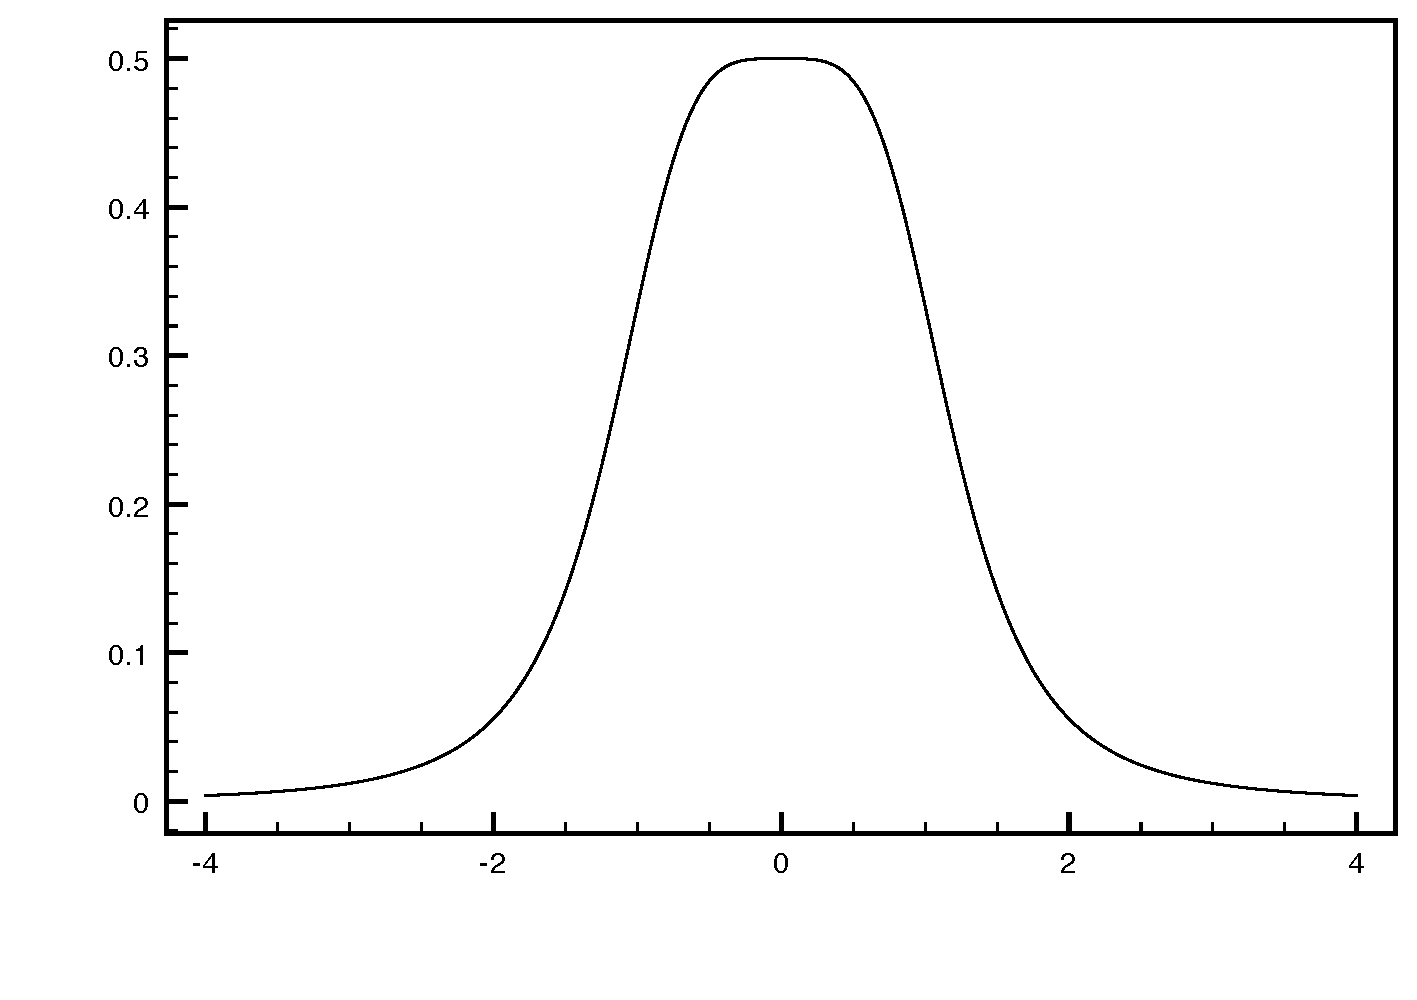
\includegraphics[width=5.15in]{Graph.pdf}
			\end{figure}	
			
		\end{enumerate}
		
	\item If $f: \mathbb{R} \rightarrow \mathbb{R}$ is differentiable and $f(x) \ne 0$ for all $x \in \mathbb{R}$,
		then by the formal definition of the derivative,
		\begin{eqnarray}
			\hspace{0.75cm} \frac{ d}{ dx} \left(\frac{1}{f(u)} \right) & = & \lim_{h\rightarrow0} \frac{\frac{1}
			{f(u+h)}- \frac{1}{f(u)}}{h} \text{ } =  \text{ } \lim_{h\rightarrow0} \text{ } \frac{f(u)-f(u+h)}{h\cdot 
			f(u+h)\cdot f(u)} \nonumber \\
			& = & -\lim_{h\rightarrow0} \text{ } \frac{\frac{f(u+h)-f(u)}{h}}{f(u+h)\cdot f(u)} \nonumber \text{ } =
			\text{ } -\frac{\lim_{h\rightarrow0} \frac{f(u+h)-f(u)}{h}}{\lim_{h\rightarrow0} f(u+h)\cdot f(u)} 
			\nonumber \\
			& = & -\frac{f'(u)}{f(u+0)\cdot f(u)} \text{ } = \text{ } -\frac{f'(u)}{f(u)\cdot f(u)} \text{ } = \text{ }
			-\frac{f'(u)}{[f(u)]^2} \nonumber
		\end{eqnarray} \\
		As $f$ is assumed differentiable at $x$, it is therefore continuous at $x$. This implies
		\begin{eqnarray}
			\hspace{2cm} \lim_{h\rightarrow0} f(u+h) = f(u) \nonumber
		\end{eqnarray}
		Meanwhile, since $f(u)$ does not involve $h$,
		\begin{eqnarray}
			\hspace{2cm} \lim_{h\rightarrow0} f(u) = f(u) \nonumber
		\end{eqnarray}
		Thus we have shown that $g: \mathbb{R} \rightarrow \mathbb{R} \text{, } \text{ } u \mapsto 
		\frac{1}{f(u)}$ is also differentiable for all $u \in \mathbb{R}$.
		
\end{enumerate}
	
\end{document}